% !TEX encoding = UTF-8 Unicode

O compilador por nós criado terá como linguagem de saída um programa que será executado na máquina virtual chamada Máquina de von Neumann (MVN).

O Modelo de von Neumann procura oferecer uma alternativa prática, disponibilizando ações mais poderosas e ágeis em seu repertório de operações que o modelo de Turing. Isso viabiliza, codificações muito mais expressivas, compactas e eficientes. Para isso, a Máquina de von Neumann utiliza:

\begin{itemize}
	\item Memória endereçável, usando acesso aleatório
	\item Programa armazenado na memória, para definir diretamente a função corrente da máquina (ao invés da Máquina de Estados Finitos)
	\item Dados representados na memória (ao invés da fita)
	\item Codificação numérica binária em lugar da unária
	\item Instruções variadas e expressivas para a realização de operações básicas muito frequentes (ao invés de sub-máquinas específicas)
	\item Maior flexibilidade para o usuário, permitindo operações de entrada e saída, comunicação física com o mundo real e controle dos modos de operação da máquina 
\end{itemize}

Dessa forma, utilizaremos essa máquina para executar nosso compilador e realizar os testes necessários.

\begin{figure}[ht]
	\centering
	\caption{Arquitetura MVN}
	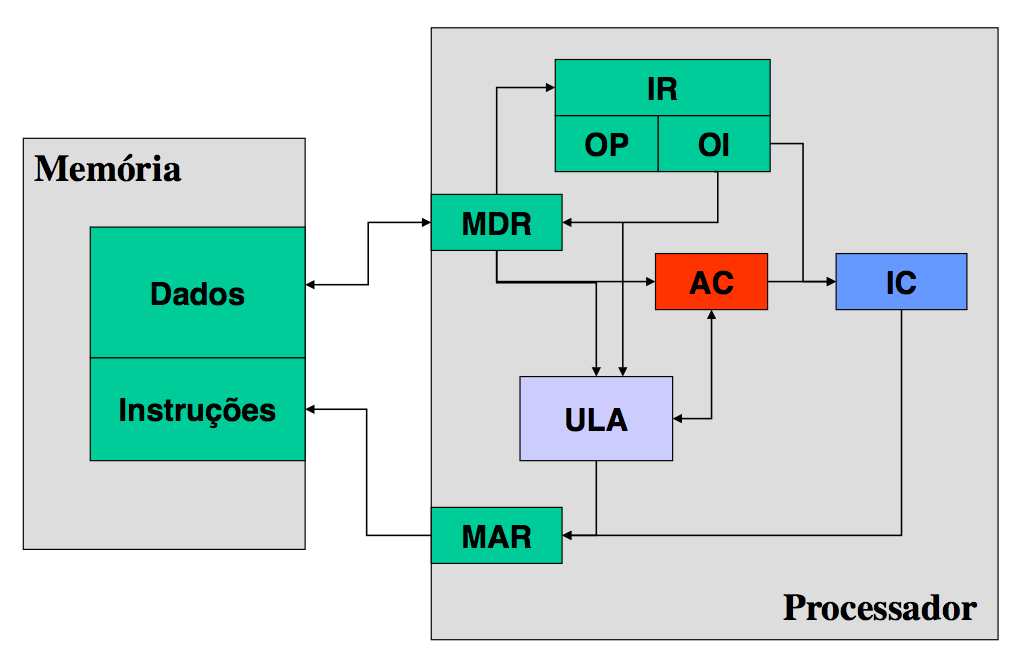
\includegraphics[width=\textwidth]{images/arquitetura-mvn.png}
	\label{fig:arquitetura-mvn}
\end{figure}

A arquitetura de Von Neumann é composta por um processador e uma memória principal. Na memória principal armazenam-se as instruções do código-fonte e os dados, sendo a divisão mostrada na figura~\ref{fig:arquitetura-mvn} apenas ilustrativa. Além da Unidade Lógica Aritmética (ULA), responsável pelo processamento de operações lógicas e aritméticas, o processador possui um conjunto de elementos físicos de armazenamento de informações e é comum dividir esses componentes nos seguintes módulos resgistradores:

\begin{enumerate}
	\item MAR - Registrador de endereço de memória
	
	Indica qual é a origem ou o destino, na memória principal, dos dados contidos no registrador de dados de memória.
	
	\item MDR -  Registrador de dados da memória
	
	Serve como ponte para os dados que trafegam entre a memória e os outros elementos da máquina.

	\item IC - Registrador de endereço de instrução 

	Indica a cada instante qual será a próxima instrução a ser executada pelo processador.

	\item IR -  Registrador de instrução

	Contém a instrução atual a ser executada. é subdividido em dois outros registradores, como na figura~\ref{fig:estrutura-ir}.
	\begin{figure}[ht]
		\centering
		\caption{Estrutura do registro de instrução (IR)}
		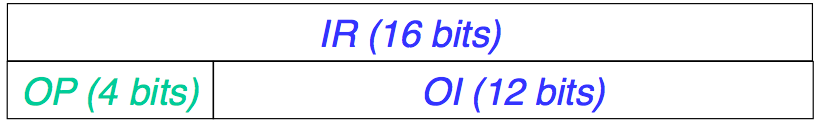
\includegraphics[width=0.8\textwidth]{images/estrutura-ir.png}
		\label{fig:estrutura-ir}
	\end{figure}

	\begin{enumerate}
		\item OP - Registrador de código de operação

		Parte do registrador de instrução que identifica a instrução que está sendo executada.

		\item OI - Registrador de operando de instrução

		Complementa a instrução indicando o dado ou o endereço sobre o qual ela deve agir.
	\end{enumerate}

	\item AC - Acumulador 

	Funciona como a área de trabalho para execução de operações lógicas ou aritméticas. Acumula o resultado de tais operações.
\end{enumerate}

A máquina executa um programa em diversos passos, listadas abaixo:

\begin{enumerate}
	\item Determinação da Próxima Instrução a Executar
	\item Fase de Obtenção da Instrução

	Obter na memória, no endereço contido no registrador de Endereço da Próxima Instrução, o código da instrução desejada.
	
	\item Fase de Decodificação da Instrução
	\label{item:decod-instrucao}

	Decompor a instrução em duas partes: o código da instrução e o seu operando, depositando essas partes nos registradores de instrução e de operando, respectivamente. Selecionar, com base no conteúdo do registrador de instrução, um procedimento de execução dentre os disponíveis no repertório do simulador (passo~\ref{item:exec-instrucao}).

	\item Fase de Execução da Instrução
	\label{item:exec-instrucao}
	
	Executar o procedimento selecionado no passo~\ref{item:decod-instrucao}, usando como operando o conteúdo do registrador de operando, preenchido anteriormente.
	
	Caso a instrução executada não seja de desvio, incrementar o registrador de endereço da próxima instrução a executar. Caso contrário, o procedimento de execução já terá atualizado convenientemente tal informação.
	
	\begin{enumerate}
		\item Execução da instrução (decodificada no passo~\ref{item:decod-instrucao})

		De acordo com o código da instrução a executar (contido no registrador de instrução), executar os procedimentos de simulação correspondentes (detalhados adiante).
		
		\item Acerto do registrador de Endereço da Próxima Instrução para apontar a próxima instrução a ser simulada:

		Incrementar o registrador de Endereço da Próxima Instrução.
	\end{enumerate}
	
\end{enumerate}


\section{Instruções da Linguagem de Saída}

As instruções da MVN podem ser resumidas pela tabela da figura~\ref{fig:instrucoes-mvn}.

\begin{figure}[ht]
	\centering
	\caption{Lista de instruções da MVN}
	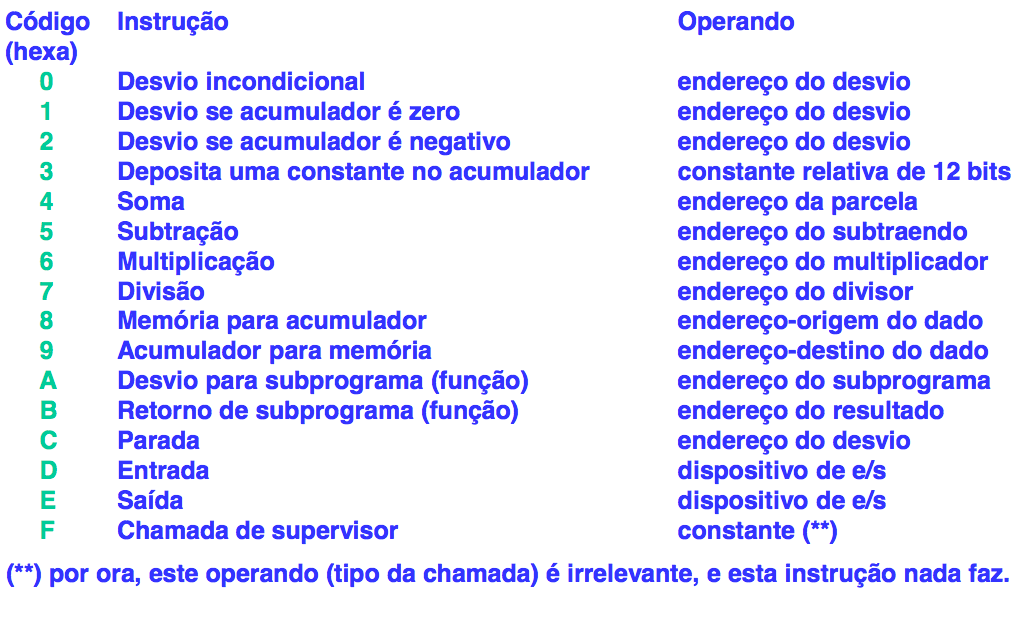
\includegraphics[width=\textwidth]{images/instrucoes-mvn.png}
	\label{fig:instrucoes-mvn}
\end{figure}

A seguir, especificaremos o que é realizado pela máquina ao executar cada tipo de operação.		

\begin{itemize}
	\item Registrador de instrução = 0 (desvio incondicional)

	Modifica o conteúdo do registrador de Endereço da Próxima Instrução (IC) armazenando nele o conteúdo do registrador de operando (OI)

	IC := OI

	\item Registrador de instrução = 1 (desvio se acumulador é zero)

	Se o conteúdo do acumulador (AC) for zero, então modifica o conteúdo do registrador de Endereço da Próxima Instrução (IC), armazenando nele o conteúdo do registrador de operando (OI) 

	Se AC = 0 então IC := OI 
	
	Se não IC := IC + 1 

	\item Registrador de instrução = 2 (desvio se negativo)

	Se o conteúdo do acumulador (AC) for negativo, isto é, se o bit mais significativo for 1, então modifica o conteúdo do registrador de Endereço da Próxima Instrução (IC) armazenando nele o conteúdo do registrador de operando (OI)

	Se AC < 0 então IC := OI 
	
	Se não IC := IC + 1

	\item Registrador de instrução = 3 (constante para acumulador)

	Armazena no acumulador (AC) o número relativo de 12 bits contido no registrador de operando (OI), estendendo seu bit mais significativo (bit de sinal) para completar os 16 bits do acumulador
		
	AC := OI 
	
	IC := IC +1 

	\item Registrador de instrução = 4 (soma)

	Soma ao conteúdo do acumulador (AC) o conteúdo da posição de memória indicada pelo registrador de operando MEM[OI]. Guarda o resultado no acumulador

	AC := AC + MEM[OI] 

	IC := IC + 1

	\item Registrador de instrução = 5 (subtração)

	Subtrai do conteúdo do acumulador (AC) o conteúdo da posição de memória indicada pelo registrador de operando MEM[OI]. Guarda o resultado no acumulador

	AC := AC - MEM[OI]

	IC := IC + 1 
		
	\item Registrador de instrução = 6 (multiplicação)

	Multiplica o conteúdo do acumulador (AC) pelo conteúdo da posição de memória indicada pelo registrador de operando MEM[OI]. Guarda o resultado no acumulador

	AC := AC * MEM[OI] 

	IC := IC + 1

	\item Registrador de instrução = 7 (divisão inteira)

	Dividir o conteúdo do acumulador (AC) pelo conteúdo da posição de memória indicada pelo registrador de operando MEM[OI]. Guarda a parte inteira do resultado no acumulador

	AC := int (AC / MEM[OI])

	IC := IC + 1 
			
	\item Registrador de instrução = 8 (memória para acumulador)

	Armazena no acumulador (AC) o conteúdo da posição de memória endereçada pelom registrador de operando (OI) 

	AC := MEM[OI]		

	IC := IC + 1
			
	\item Registrador de instrução = 9 (acumulador para memória)

	Guarda o conteúdo do acumulador (AC) na posição de memória endereçada pelo registrador de operando (OI) 

	MEM[OI] := AC		
	
	IC := IC + 1 
			
	\item Registrador de instrução = A (desvio para subprograma)

	Armazena o conteúdo do registrador de Endereço da Próxima Instrução (IC), incrementado de uma unidade, no registrador de endereço de retorno (RA). Armazena no registrador de Endereço da Próxima Instrução (IC) o conteúdo do registrador de operando (OI).

	RA := IC + 1
	
	IC := OI

	\item Registrador de instrução = B (retorno de subprograma)

	Armazena no registrador de Endereço da Próxima Instrução (IC) o conteúdo do registrador de endereço de retorno (RA), e no acumulador (AC) o conteúdo da posição de memória apontada pelo registrador de operando (OI) 

	AC := MEM[OI]			

	IC := RA 	 	 	 		

			
	\item Registrador de instrução = C (stop)

	Modifica o conteúdo do registrador de Endereço da Próxima Instrução (IC) armazenando nele o conteúdo do registrador de operando (OI) e para o processamento

	IC := OI

	\item Registrador de instrução = D (input)
 					
	Aciona o dispositivo padrão de entrada e aguardar que o usuário forneça o próximo dado a ser lido. Transfere o dado para o acumulador 

	Aguarda
	
	AC := dado de entrada 
	
	IC := IC + 1 
		
	\item Registrador de instrução = E (output)

	Transfere o conteúdo do acumulador (AC) para o dispositivo padrão de saída. Aciona o dispositivo padrão de saída e aguardar que este termine de executar a operação de saída 

	dado de saída := AC 

	aguarda
	
	IC := IC + 1

	\item Registrador de instrução = F (supervisor call)

	Não implementado: por enquanto esta instrução não faz nada.

	IC := IC + 1
\end{itemize}

Escrever um programa usando diretamente codificação binária não é uma tarefa simples, e tampouco agradável. Naturalmente, se um programa é muito grande ou se lida com diversas estruturas complexas (listas, etc.), a sua codificação se torna ainda mais difícil e complexa.

Por conta disso, torna-se imprescindível construir alguma abstração que facilite a programação e a verificação dos programas. A primeira idéia, mais natural, é utilizar o modelo de máquina existente e, a partir dele, definir nomes (mnemônicos) para cada instrução da máquina. Posteriormente, verifica-se que somente isso não basta, pois é necessário lidar com os endereços dentro de um programa (rótulos, operandos, sub-rotinas), com a reserva de espaço para tabelas, com valores constantes. Enfim, é necessário definir uma linguagem simbólica.

\begin{figure}[ht]
	\centering
	\caption{Esquema geral de um montador}
	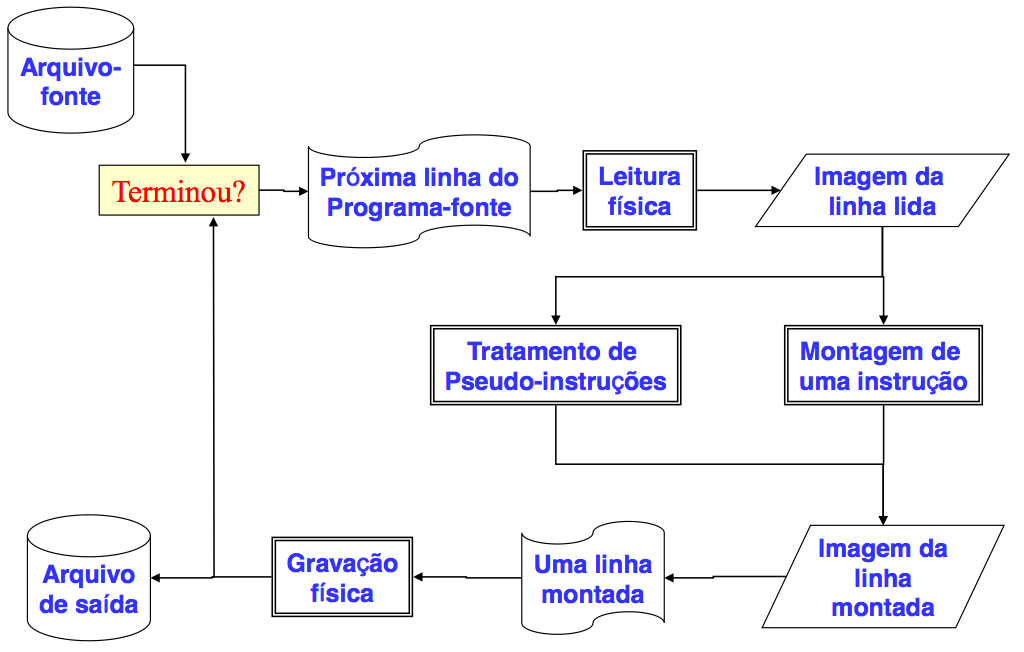
\includegraphics[width=\textwidth]{images/esquema-montador.png}
	\label{fig:esquema-montador}
\end{figure}

Para a construção de um montador, cujo esquema geral está representado na figura~\ref{fig:esquema-montador} pressupõe-se que sejam tratadas as seguintes questões:

\begin{itemize}
	\item definição das instruções: determinar os mnemônicos que as representam simbolicamente;
	\item definição das pseudo-instruções: determinar os mnemônicos que as representam, bem como sua função para o montador.
\end{itemize}

As instruções para a MVN são apresentadas na figura~\ref{fig:mnemonicos-mvn}.

\begin{figure}[ht]
	\centering
	\caption{Tabela de mnemônicos para a MVN (de 2 caracteres)}
	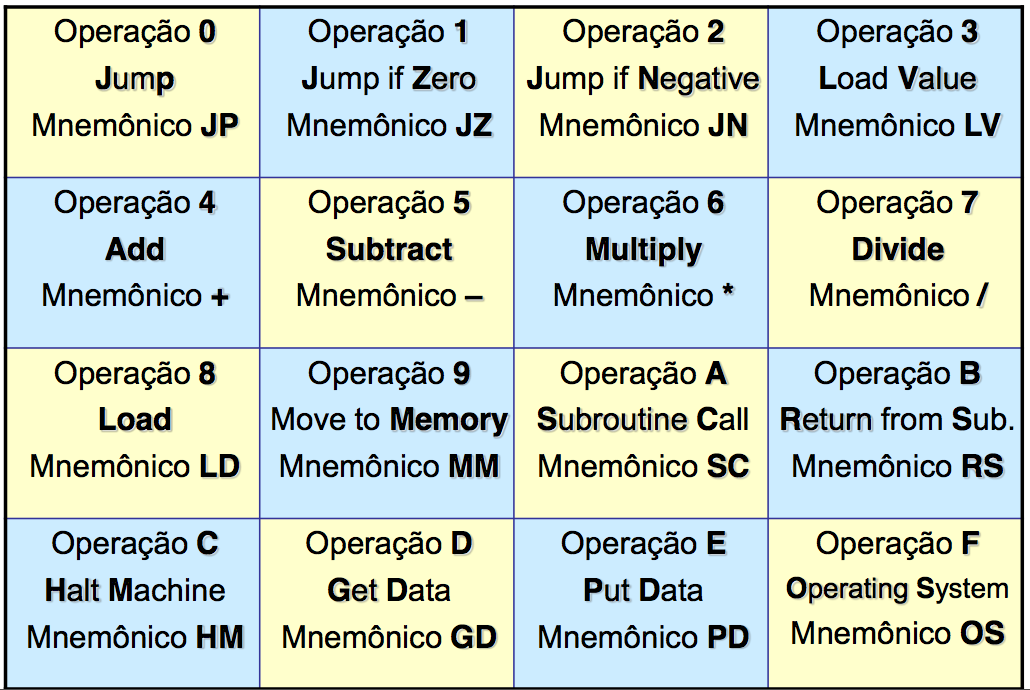
\includegraphics[width=\textwidth]{images/mnemonicos-mvn.png}
	\label{fig:mnemonicos-mvn}
\end{figure}


\section{Pseudoinstruções da Linguagem de Saída}

Programas absolutos são executáveis estritamente nas posições de memória em que foram criados, tornando difícil a manutenção e o trabalho em equipe. A utilização de programas relocáveis permitem sua execução em qualquer posição de memória, tornando possível utilizar partes de código projetadas externamente (uso de bibliotecas, por exemplo).

Para que se possa exprimir um programa relocável e com possibilidade de construção em módulos, separadamente desenvolvidos, é necessário que:
\begin{itemize}
	\item Haja a possibilidade de representar e identificar endereços absolutos e endereços relativos;
	\item Um programa possa ser montado sem que os seus endereços simbólicos estejam todos resolvidos;
	\item Seja possível identificar, em um módulo, símbolos que possam ser referenciados simbolicamente em outros módulos.
\end{itemize}

Sendo assim, a linguagem simbólica não possui somente os mnemônicos das instruções da MVN, mas também comandos chamados de pseudo-instruções da linguagem de montagem. Na linguagem de montagem, as pseudo-instruções também são representadas por mnemônicos, listados abaixo:

\begin{itemize}
	\item @ : Origem Absoluta. Recebe um operando numérico, define o endereço da instrução seguinte;
	\item K : Constante, o operando numérico tem o valor da constante (em hexadecimal). Define uma área preenchida por uma CONSTANTE de 2 bytes;
	\item \$ : Reserva de área de dados, o operando numérico define o tamanho da área a ser reservada. Define um BLOCO DE MEMóRIA com número especificado de words;
	\item \# : Final físico do texto fonte;
	\item \& : Origem relocável;
	\item > : Endereço simbólico de entrada (entry point). Define um endereço simbólico local como entry-point do programa;
	\item < : Endereço simbólico externo (external). Define um endereço simbólico que referencia um entry-point externo.
\end{itemize}

Na figura~\ref{fig:exemplo-somador}, temos um exemplo de um somador escrito em linguagem de montagem, visto na aula de Fundamentos de Eng. de Computação, e sua respectiva tradução pelos módulos Montador, \emph{Linker} e Relocador, módulos extras porém integrados no nosso caso:

\begin{figure}[ht]
	\centering
	\caption{Exemplo de um somador}
	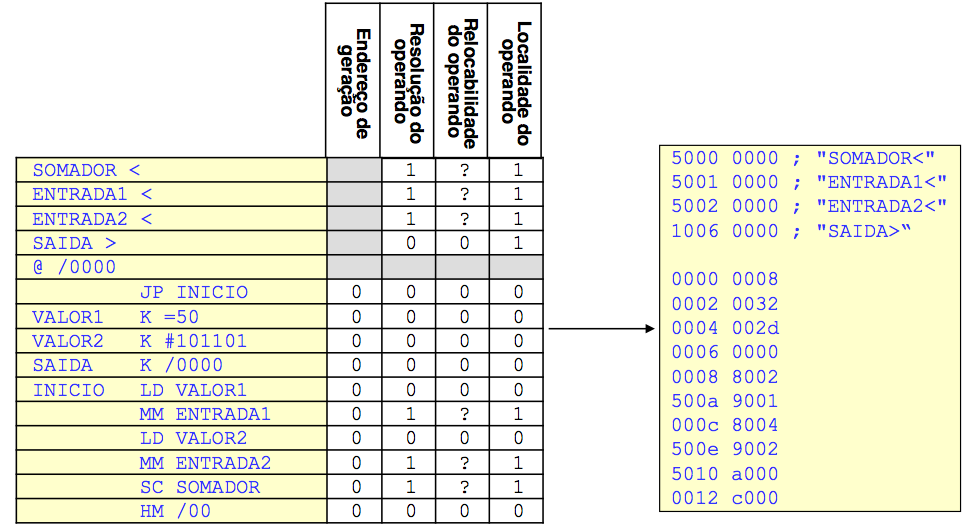
\includegraphics[width=\textwidth]{images/exemplo-somador.png}
	\label{fig:exemplo-somador}
\end{figure}

